
\documentclass[border=10pt, 12pt]{standalone}
\usepackage[svgnames]{xcolor}
\usepackage{amsmath}
\usepackage{pgfplots}
\pgfplotsset{compat=newest}
\usepackage[sfdefault]{FiraSans}
\usepackage{FiraMono}
\renewcommand*\familydefault{\sfdefault}
\begin{document}
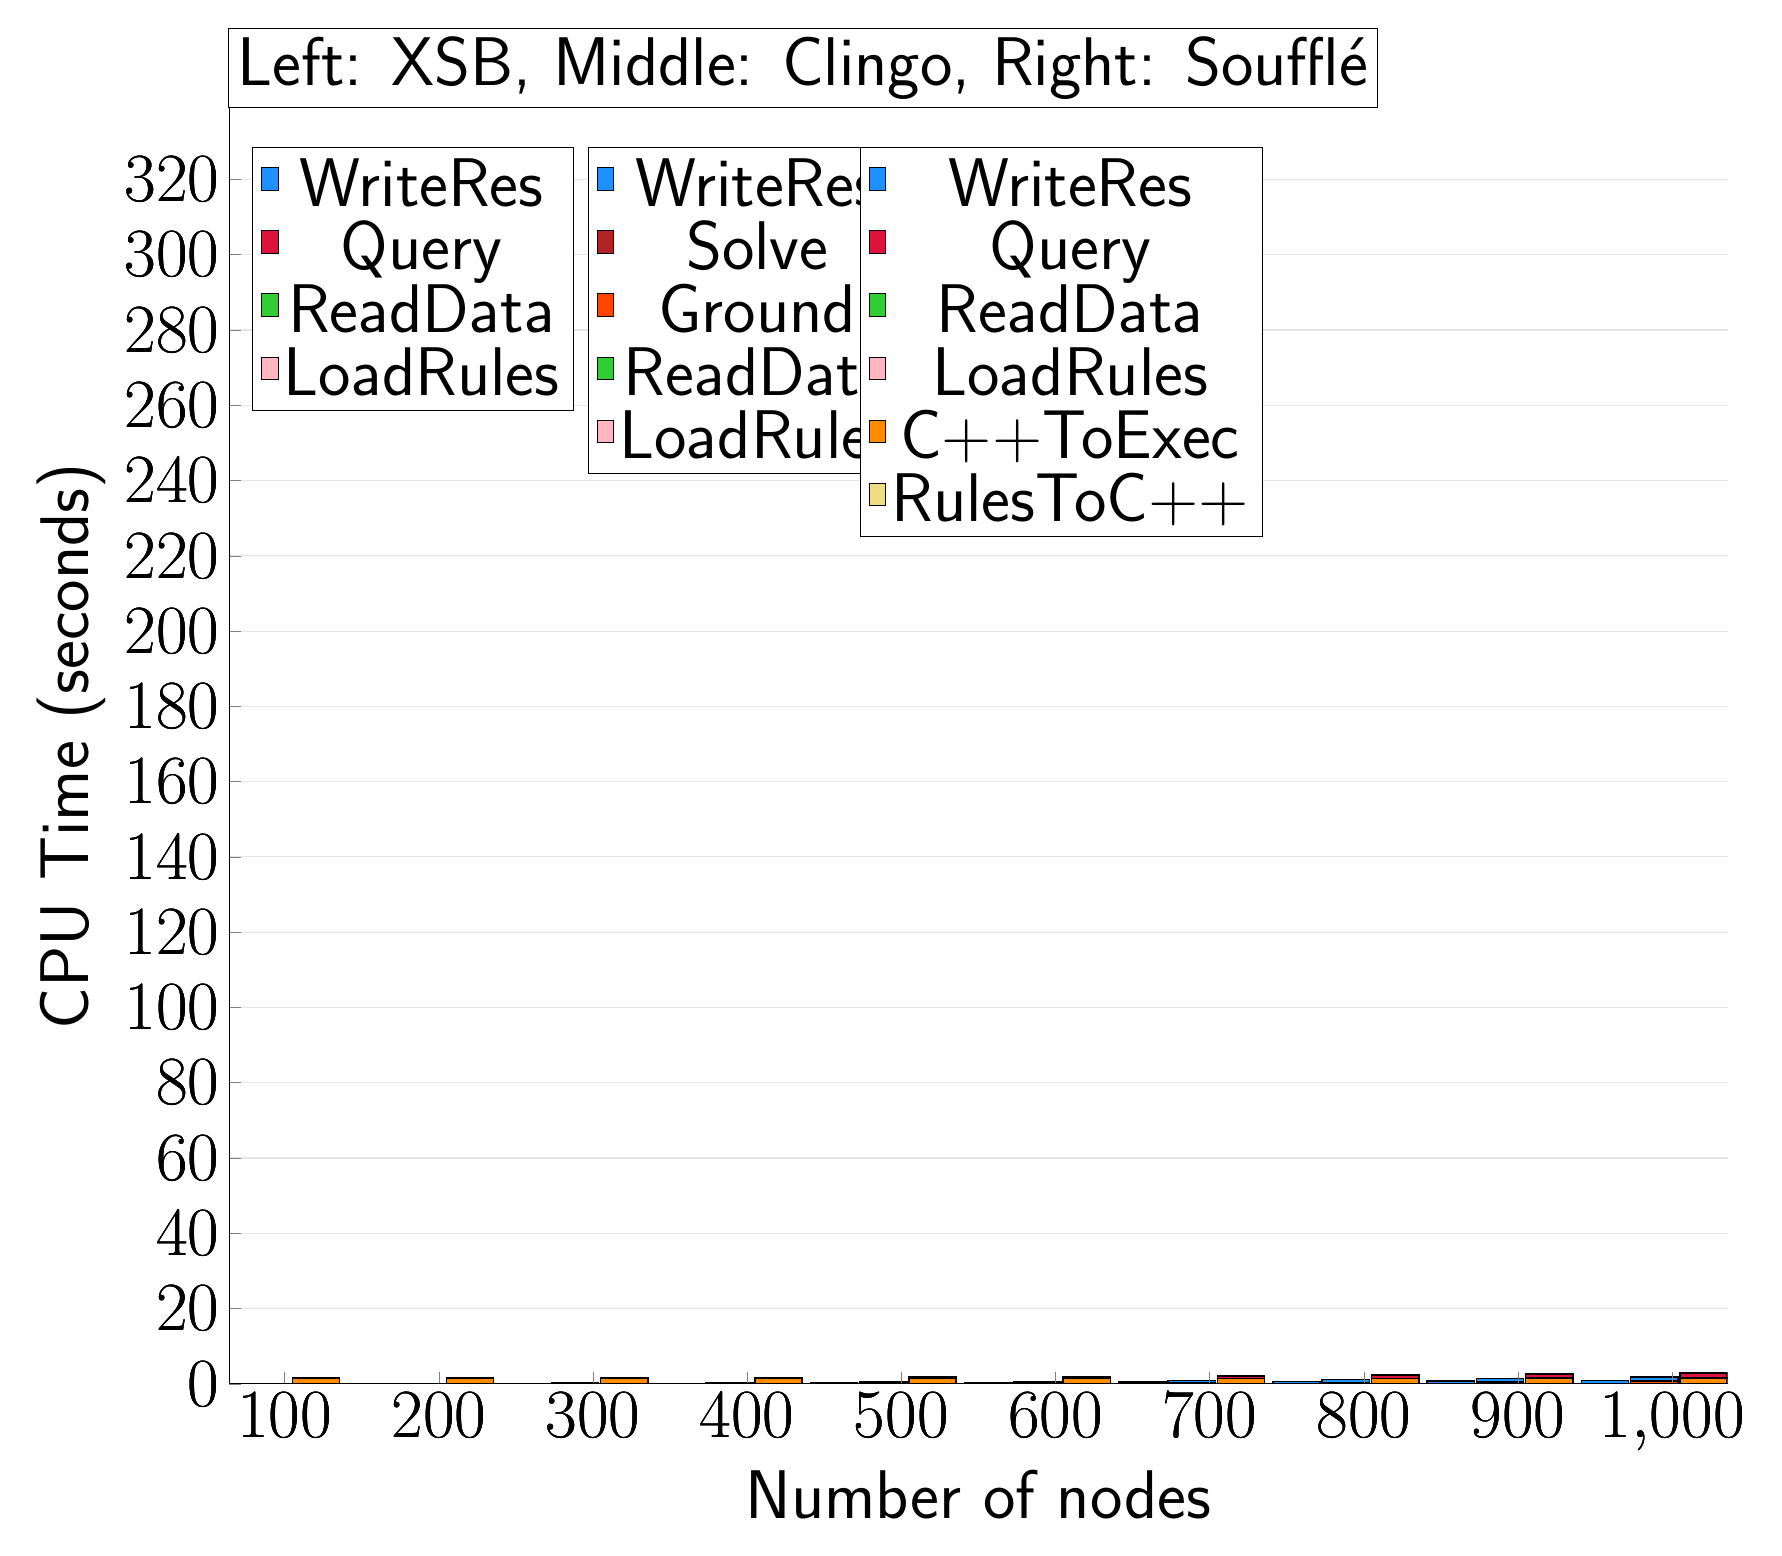
\begin{tikzpicture}
                        \begin{axis}[bar shift=-24.3pt, 
   ybar stacked,
   width=1.7\textwidth,
   bar width=0.6cm,
   ymajorgrids, tick align=inside,
   major grid style={draw=gray!20},
   xtick=data,
   ymin=0, ymax=338.8692,
   axis x line*=bottom,
   axis y line*=left,
   enlarge x limits=0.04,
   legend style={
       at={(0.23, 0.97)},
       anchor=north east,
       legend columns=1,
       font=\Huge,
   },
   ylabel={CPU Time (seconds)},
   xlabel={Number of nodes},
   label style={font=\Huge},
   tick label style={font=\Huge},
]
\addlegendimage{fill=DodgerBlue, draw=black, line width=0.2pt}
\addlegendentry{WriteRes}
\addlegendimage{fill=Crimson, draw=black, line width=0.2pt}
\addlegendentry{Query}
\addlegendimage{fill=LimeGreen, draw=black, line width=0.2pt}
\addlegendentry{ReadData}
\addlegendimage{fill=LightPink, draw=black, line width=0.2pt}
\addlegendentry{LoadRules}
\addplot +[fill=LightPink, draw=black, line width=0.55pt] coordinates {
(100, 0.0005588000000000005)
(200, 0.0005505999999999996)
(300, 0.0005531999999999994)
(400, 0.0005576000000000002)
(500, 0.0005535999999999994)
(600, 0.0005506)
(700, 0.0005583999999999996)
(800, 0.0005560000000000002)
(900, 0.0005509999999999994)
(1000, 0.0005509999999999998)
};
\addplot +[fill=LimeGreen, draw=black, line width=0.55pt] coordinates {
(100, 0.00019580000000000018)
(200, 0.00028100000000000043)
(300, 0.00035339999999999997)
(400, 0.0004368000000000002)
(500, 0.000514800000000001)
(600, 0.000597)
(700, 0.0006764)
(800, 0.0007526)
(900, 0.0008260000000000006)
(1000, 0.0008982)
};
\addplot +[fill=Crimson, draw=black, line width=0.55pt] coordinates {
(100, 0.0008719999999999998)
(200, 0.0035654000000000007)
(300, 0.0083158)
(400, 0.0159714)
(500, 0.024759999999999997)
(600, 0.036933799999999996)
(700, 0.0499226)
(800, 0.0653826)
(900, 0.0824588)
(1000, 0.10194639999999999)
};
\addplot +[fill=DodgerBlue, draw=black, line width=0.55pt] coordinates {
(100, 0.0081424)
(200, 0.032930799999999996)
(300, 0.07388299999999999)
(400, 0.1300476)
(500, 0.2035558)
(600, 0.2907868)
(700, 0.39730360000000003)
(800, 0.519544)
(900, 0.6500966)
(1000, 0.8040232000000002)
};
\end{axis}

\begin{axis}[bar shift=-6.5pt, 
   ybar stacked,
   width=1.7\textwidth,
   bar width=0.6cm,
   ymajorgrids, tick align=inside,
   major grid style={draw=none},
   xtick=data,
   ymin=0, ymax=338.8692,
   axis x line*=none,
   axis y line*=none,
   enlarge x limits=0.04,
   legend style={
       at={(0.454, 0.97)},
       anchor=north east,
       legend columns=1,
       font=\Huge,
   },
   label style={font=\Huge},
   tick label style={font=\Huge},
]
\addlegendimage{fill=DodgerBlue, draw=black, line width=0.2pt}
\addlegendentry{WriteRes}
\addlegendimage{fill=FireBrick, draw=black, line width=0.2pt}
\addlegendentry{Solve}
\addlegendimage{fill=OrangeRed, draw=black, line width=0.2pt}
\addlegendentry{Ground}
\addlegendimage{fill=LimeGreen, draw=black, line width=0.2pt}
\addlegendentry{ReadData}
\addlegendimage{fill=LightPink, draw=black, line width=0.2pt}
\addlegendentry{LoadRules}
\addplot +[fill=LightPink, draw=black, line width=0.55pt] coordinates {
(100, 0.0)
(200, 0.0)
(300, 0.0)
(400, 0.0)
(500, 0.0)
(600, 0.0)
(700, 0.0)
(800, 0.0)
(900, 0.0)
(1000, 0.0)
};
\addplot +[fill=LimeGreen, draw=black, line width=0.55pt] coordinates {
(100, 0.0)
(200, 0.0)
(300, 0.0)
(400, 0.0)
(500, 0.0)
(600, 0.0)
(700, 0.0)
(800, 0.0)
(900, 0.0)
(1000, 0.0)
};
\addplot +[fill=OrangeRed, draw=black, line width=0.55pt] coordinates {
(100, 0.0)
(200, 0.020000000000000018)
(300, 0.04999999999999999)
(400, 0.08800000000000002)
(500, 0.14400000000000002)
(600, 0.21000000000000002)
(700, 0.29400000000000004)
(800, 0.376)
(900, 0.48)
(1000, 0.622)
};
\addplot +[fill=FireBrick, draw=black, line width=0.55pt] coordinates {
(100, 0.0)
(200, 0.0)
(300, 0.0)
(400, 0.006000000000000004)
(500, 0.016000000000000014)
(600, 0.020000000000000018)
(700, 0.030000000000000034)
(800, 0.03600000000000003)
(900, 0.05800000000000004)
(1000, 0.062000000000000055)
};
\addplot +[fill=DodgerBlue, draw=black, line width=0.55pt] coordinates {
(100, 0.014000000000000012)
(200, 0.04999999999999999)
(300, 0.11000000000000006)
(400, 0.194)
(500, 0.2879999999999999)
(600, 0.41600000000000004)
(700, 0.5699999999999998)
(800, 0.7339999999999999)
(900, 0.914)
(1000, 1.14)
};
\end{axis}

\begin{axis}[bar shift=11.3pt, 
   ybar stacked,
   width=1.7\textwidth,
   bar width=0.6cm,
   ymajorgrids, tick align=inside,
   major grid style={draw=none},
   xtick=data,
   ymin=0, ymax=338.8692,
   axis x line*=none,
   axis y line*=none,
   enlarge x limits=0.04,
   legend style={
       at={(0.69, 0.97)},
       anchor=north east,
       legend columns=1,
       font=\Huge,
   },
   label style={font=\Huge},
   tick label style={font=\Huge},
]
\addlegendimage{fill=DodgerBlue, draw=black, line width=0.2pt}
\addlegendentry{WriteRes}
\addlegendimage{fill=Crimson, draw=black, line width=0.2pt}
\addlegendentry{Query}
\addlegendimage{fill=LimeGreen, draw=black, line width=0.2pt}
\addlegendentry{ReadData}
\addlegendimage{fill=LightPink, draw=black, line width=0.2pt}
\addlegendentry{LoadRules}
\addlegendimage{fill=DarkOrange, draw=black, line width=0.2pt}
\addlegendentry{C++ToExec}
\addlegendimage{fill=LightGoldenrod, draw=black, line width=0.2pt}
\addlegendentry{RulesToC++}
\addplot +[fill=LightGoldenrod, draw=black, line width=0.55pt] coordinates {
(100, 0.0020000000000000005)
(200, 0.006000000000000001)
(300, 0.0020000000000000005)
(400, 0.0020000000000000005)
(500, 0.004000000000000001)
(600, 0.004000000000000001)
(700, 0.004000000000000001)
(800, 0.009999999999999998)
(900, 0.004000000000000001)
(1000, 0.008000000000000002)
};
\addplot +[fill=DarkOrange, draw=black, line width=0.55pt] coordinates {
(100, 1.48)
(200, 1.4739999999999998)
(300, 1.488)
(400, 1.482)
(500, 1.478)
(600, 1.478)
(700, 1.466)
(800, 1.4620000000000002)
(900, 1.4880000000000002)
(1000, 1.504)
};
\addplot +[fill=LightPink, draw=black, line width=0.55pt] coordinates {
(100, 0.0001692)
(200, 0.00016879999999999998)
(300, 0.000182)
(400, 0.0001746)
(500, 0.000169)
(600, 0.000168)
(700, 0.00016380000000000002)
(800, 0.00016439999999999998)
(900, 0.000166)
(1000, 0.0001592)
};
\addplot +[fill=LimeGreen, draw=black, line width=0.55pt] coordinates {
(100, 0.0007474)
(200, 0.0012067999999999998)
(300, 0.0016281999999999998)
(400, 0.0019854)
(500, 0.0023794000000000003)
(600, 0.0027480000000000004)
(700, 0.0028266000000000003)
(800, 0.0027815999999999995)
(900, 0.0037388000000000005)
(1000, 0.0029401999999999996)
};
\addplot +[fill=Crimson, draw=black, line width=0.55pt] coordinates {
(100, 0.020999999999999998)
(200, 0.06437040000000001)
(300, 0.1214092)
(400, 0.20174659999999997)
(500, 0.3090962)
(600, 0.4413768)
(700, 0.5979896)
(800, 0.7903472)
(900, 1.006362)
(1000, 1.2769679999999999)
};
\addplot +[fill=DodgerBlue, draw=black, line width=0.55pt] coordinates {
(100, 0.0038366)
(200, 0.009382600000000001)
(300, 0.019478600000000002)
(400, 0.034334199999999995)
(500, 0.053332000000000004)
(600, 0.07630279999999999)
(700, 0.1045544)
(800, 0.137103)
(900, 0.1708554)
(1000, 0.21426239999999996)
};
\end{axis}


\node[anchor=south, draw, fill=white] at (rel axis cs:0.42,1) {\Huge Left: XSB, Middle: Clingo, Right: Soufflé};
\end{tikzpicture}
\end{document}
                    